\subsection{Cryptographic Keys}\label{sec:cryptography_basics:keys}

A \textbf{cryptographic key} (or simply key) is usually one of the inputs of a cryptographic algorithm (\Cref{sec:cryptography_basics:algorithms}) that determines its operation such that an entity possessing the key can reproduce, invert, or verify the operation, whereas an entity without the key cannot \cite{barker_recommendation_2020_p1}. A key may be either a (carefully chosen or generated) meaningless sequence of bytes --- as in symmetric cryptography (\Cref{sec:symmetric_cryptography}) --- or a tuple of one or more mathematically related elements or structures (e.g., integer numbers, points on elliptic curves, isogenies) --- as in asymmetric cryptography (\Cref{sec:asymmetric_cryptography}). The length of a key in bits is usually called \textbf{key length} or \textit{key size}.

A key used in symmetric cryptography is called \textbf{symmetric key}. Generally, symmetric keys are known by one party (e.g., when protecting data at rest) or, more frequently, by a specific set of two or more parties (e.g., when protecting data in transit). Symmetric keys are also called \textit{secret keys} or \textit{shared keys} --- when known by more than one party. 

\warningBlock{Ambiguous names for symmetric keys}{Symmetric keys are sometimes called \textit{shared secrets} which, however, may be an ambiguous term as it is used in other contexts as well. For instance, the output of \gls{dh} key agreements is also called shared secret --- see \Cref{sec:diffie_hellman}.}

A key used in asymmetric cryptography is called \textbf{asymmetric key}. Asymmetric cryptography typically employs two kinds of keys: \textbf{public keys} and \textbf{private keys}. By definition, a public key can be publicly disclosed and known by anyone within a system. Conversely, a private key is (almost\footnote{``Almost'' because some cryptographic constructions --- e.g., \gls{ibe}
%TODO (\Cref{future_sec:identity_based_cryptography}) 
and \gls{abe} 
%TODO (\Cref{future_sec:advanced_cryptography:attribute_based_encryption})
--- private keys are actually generated by a trusted party called \textbf{\gls{kga}}. Typically, after having generated a private key and shared it with the owner, the \gls{kga} should forget the private key (e.g., delete it from memory).}) always known by one party only corresponding to the owner of the key. A private key is always related to exactly one public key, either mathematically (i.e., by design) or by embedding random values used to uniquely derive the corresponding public key. However, \textit{it must be computationally infeasible to derive a private key from the corresponding public key}. Conversely, it is usually possible to derive a public key from the corresponding private key. A private key and a public key are (almost\footnote{``Almost'' because in some cryptographic constructions --- again, like \gls{ibe} and \gls{abe} --- it is possible that more private keys are assigned to the same public key.}) always exclusively assigned to each other and form a \textbf{key pair}. Public and private keys may be generated together or at a different point in time (usually, the private key is generated after the public key).

Depending on its origin or use, keys may be:

\begin{itemize}
	\item \textbf{ephemeral}, that is, freshly generated when needed and immediately disposed of after being used once. The use of ephemeral keys provides forward secrecy (\Cref{sec:security_properties}) and --- to some extent (but not necessarily) --- protection against replay attacks (\Cref{sec:security_of_cryptographic_protocols}). Ephemeral keys are usually asymmetric keys and are often used in the \gls{dh} key agreement (\Cref{sec:diffie_hellman});
	\item \textbf{short-term}, that is, freshly generated when needed and disposed of after being used for a limited number of times or period (e.g., in the order of minutes, hours, or a few days). Short-term keys are usually symmetric keys used for protecting data in transit within communications;
	\item \textbf{long-term}, that is, not ephemeral. Long-term keys are also called \textbf{static} and are often --- though not necessarily --- bonded to parties through either a \gls{pki} or the \gls{wot} (\Cref{sec:binding_keys_to_parties,sec:binding_keys_to_parties:wot}, respectively);
	\item \textbf{\glspl{dek}}, that is, keys used specifically to en/decrypt data. \glspl{dek} are almost always symmetric keys. Reusing the same \gls{dek} to encrypt distinct pieces of data is usually discouraged (so to limit the impact of the loss or leak of the \gls{dek});
	\item \textbf{\glspl{kek}}, that is, keys used specifically to en/decrypt other keys. \glspl{kek} may be both symmetric or asymmetric keys;
	\item \textbf{main keys},\footnote{As adopted by other authoritative sources such as the \gls{nist} \cite{hu_overview_2023}, in an effort to address biased language we prefer the use of ``main'' over ``master'' (and ``slave'').} which is an ambiguous term that may refer to:
	\begin{itemize}
		\item \textbf{main (\gls{kek}) keys}, that is, \glspl{kek} which are never encrypted with other \glspl{kek} --- although main keys are protected, usually with dedicated software (e.g., keystores) or --- better --- hardware (\Cref{sec:cryptographic_modules});
		\item \textbf{main (generation) keys}, that is, private keys hold by \glspl{kga} used to generate other private keys, usually in the context of cryptosystems based on bilinear pairings (\Cref{sec:trapdoor_functions:elliptic_curve_cryptography:pairings}) such as \gls{abe};
	\end{itemize}
	\item \textbf{weak keys}, that is, keys that make specific cryptographic algorithms behave in some undesirable (and insecure) way. Weak keys usually represent a very small fraction of the possible keys and (obviously) should be avoided.
\end{itemize}

\remarkBlock{Key wrapping and envelope encryption}{The practice of encrypting keys with \glspl{kek} is called \textbf{key wrapping}, while the practice of encrypting data with \glspl{dek} and then encrypting \glspl{dek} with \gls{kek} --- usually in the context of hybrid cryptography (\Cref{sec:hybrid_cryptography}) --- is called \textbf{envelope encryption}.}

\paragraph*{Key Generation.} The process of generating keys usually consists of a protocol whereby one or more keys are created or derived by one or more interacting parties --- please refer to \Cref{sec:key_management:lifecycle:pre} for more information on protocols for key generation. At a high level, all keys should be generated:

\begin{itemize}
	\item to be \textbf{suitable for use in the intended purpose and application}. For instance, a symmetric key cannot be used in asymmetric cryptography. Similarly, a key generated for a specific cryptographic algorithm usually cannot (and must definitely not) be used as input for a different cryptographic algorithm;
	\item with a \textbf{proper length} as to render guessing attacks computationally infeasible (\Cref{sec:cryptographic_security_overview:attacks});
	\item starting from a \textbf{high entropy} (i.e., high randomness or unpredictability) source --- in the sense of being predictable by attackers with negligible probability. Hardware-based random bit generators are usually used as high entropy source.
	\curiosityBlock{Can anything be used as a high entropy source?}{The renowned CloudFlare company relies on the random movement of lava lamps (\Cref{figure:lava_lamps}) as a source of high entropy.\footnote{How do lava lamps help with Internet encryption? | Cloudflare (\url{https://www.cloudflare.com/learning/ssl/lava-lamp-encryption/})} For more details on entropy sources, we refer the interested reader to \cite{barker_recommendation_800_900_2015,turan_recommendation_2018}.}
\end{itemize}

\begin{figure}[t!]
	\begin{center}
		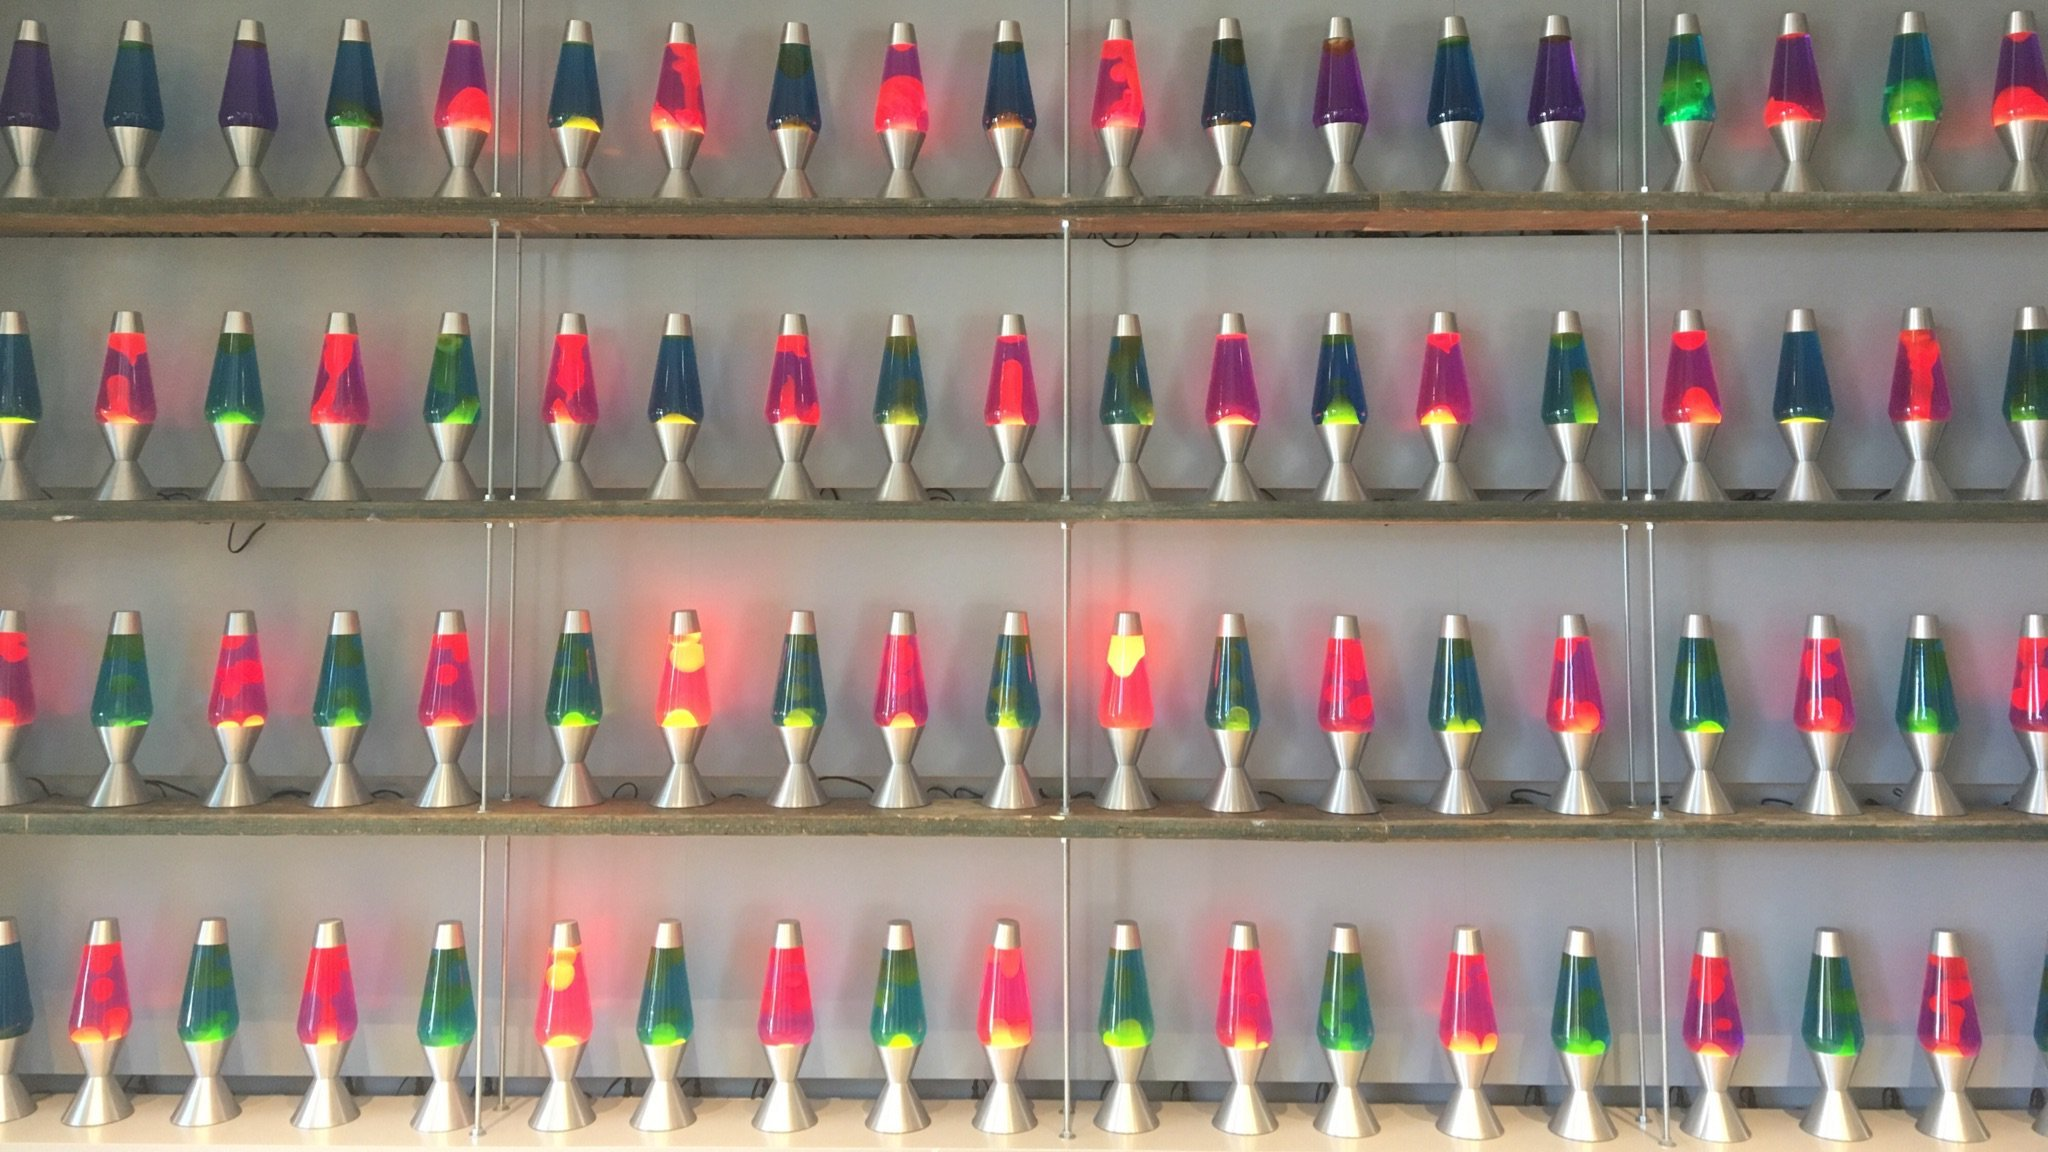
\includegraphics[width=1\linewidth]{resources/img/lava-lamps.jpg}
		\caption{Part of the 100 lava lamps in the atrium of Cloudflare's headquarters (from \url{https://www.cloudflare.com/learning/ssl/lava-lamp-encryption/})}
		\label{figure:lava_lamps}
	\end{center}
\end{figure}

Please refer to \Cref{sec:key_management} for more information on key management.